\textbf{COLUNI 2020 -- Questão 33}\par\medskip Observe e analise o gráfico abaixo.

% COLUNI-AUTO-FIGURES-BEGIN
\begin{figure}[htbp]
\centering
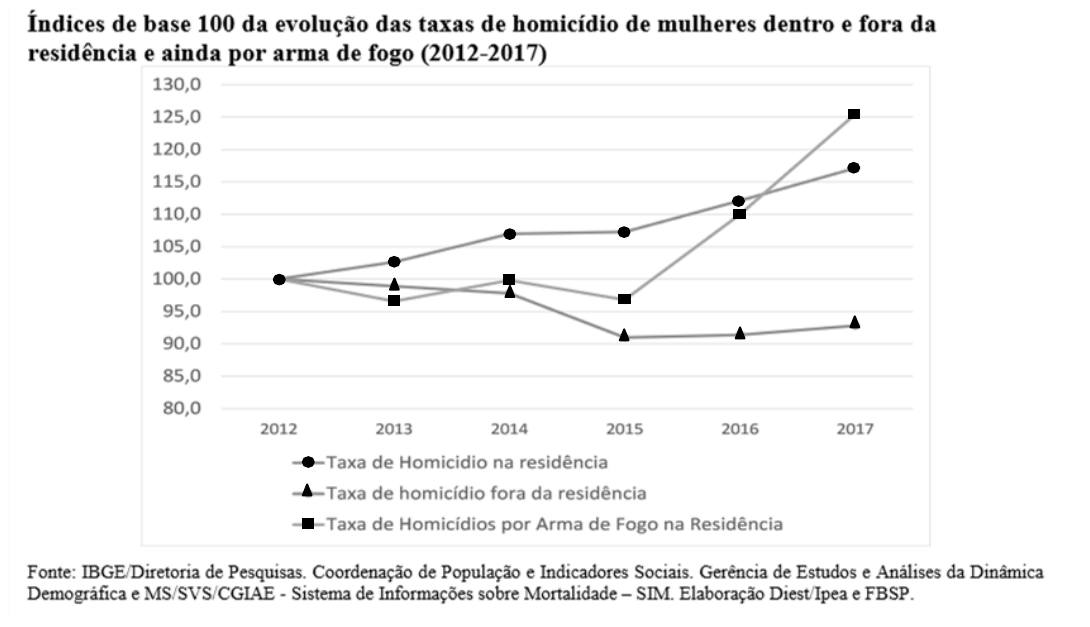
\includegraphics[width=0.95\linewidth]{static/simulados/coluni/figuras/2020/questao-33/figura-1.png}
\end{figure}
% COLUNI-AUTO-FIGURES-END

\par

Disponível em: http://www.ipea.gov.br/portal/images/stories/PDFs/relatorio\_institucional/190605\_atlas\_da\_violencia\_2019.pdf. Acesso em: 18 set. 2019.

\par

Com base no gráfico acima, é INCORRETO afirmar que:


\begin{enumerate}
\item a taxa de mulheres mortas por arma de fogo na residência cresceu entre 2015 e 2017.
\item o aumento da taxa de homicídios de mulheres por uso da arma de fogo deve-se a assaltos.
\item a taxa de mulheres mortas fora da residência diminuiu no ano de 2015.
\item o ano de 2014 foi o menos significativo no aumento das taxas de homicídio de mulheres.\end{enumerate}
